% REMEMBER: You must not plagiarise anything in your report. Be extremely careful.
\documentclass{l4proj}
\let\Bbbk\relax
\usepackage{pdfpages} % if you want to include a PDF for an ethics checklist, for example

%
%

\begin{document}

%==============================================================================
%% METADATA
\title{Automated Generation of Difficulty-Controlled LZW Exercises and Solutions for an Algorithms Course}
\author{Andrew King}
\date{March 27, 2026}

\maketitle

%==============================================================================
%% ABSTRACT
\begin{abstract}
Online and hybrid exams make it challenging to provide each student with a unique question without introducing differences in difficulty. This project introduces an automated generator for LZW compression and decompression exercises that addresses this by generating unique questions of consistent difficulty. The generator employs a generate-and-filter approach to target a specific step count and dictionary size for each exercise. It also supports two difficulty profiles, producing strings that feel easier or harder to trace while keeping the written workload identical. Testing demonstrated that step counts were perfectly consistent within batches, students rated the exercises as clear and comparable to class examples, and a usability study confirmed that the interface was intuitive and that the two profiles genuinely felt different in difficulty.
\end{abstract}

%==============================================================================
%% ACKNOWLEDGEMENTS
\chapter*{Acknowledgements}
I would like to thank my supervisor, Dr.\ Oana Andrei, for her guidance and support throughout this project, and for arranging access to a class test which made the evaluation possible.


%==============================================================================

% EDUCATION REUSE CONSENT FORM
% If you consent to your project being shown to future students for educational purposes
% then insert your name and the date below to  sign the education use form that appears in the front of the document. 
% You must explicitly give consent if you wish to do so.
% If you sign, your project may be included in the Hall of Fame if it scores particularly highly.
%
% Please note that you are under no obligation to sign 
% this declaration, but doing so would help future students.
%
%\def\consentname {My Name} % your full name
%\def\consentdate {20 March 2018} % the date you agree
%
\educationalconsent


\tableofcontents


\chapter{Introduction}
\pagenumbering{arabic}
 
\section{Motivation}
 
Online assessment became a necessity during the COVID-19 pandemic, and while universities have largely returned to in-person examinations, many computing science courses continue to rely on online or hybrid assessment formats due to scheduling constraints, venue availability, and student preference \citep{Chirumamilla21}. This shift exposes a key problem not associated with in person written exams. If every student receives the same paper, there is a higher risk of collusion, but creating different papers manually is both time-consuming and creates the need to calibrate the difficulty to maintain fairness across the different papers.
 
Automated exercise generation can help solve this problem by creating unique question papers, so that each student receives a different version of the same exercise. However, purely random generation can lead to questions with very different difficulty levels, which raises fairness concerns if some students receive harder papers than others. An effective generator therefore needs to strike a balance: the questions should be varied enough to discourage collusion, but overall similar enough in difficulty to keep the assessment fair.
 
Previous work has explored automated generation for satisfiability problems \citep{Hoz21}, embedded systems modelling \citep{Sad12}, and data science exercises \citep{Kot19}, and prior work at the University of Glasgow \citep{PriorGlasgow} has investigated generation for graph and string algorithms, specifically Dijkstra's shortest-path algorithm and the Knuth--Morris--Pratt string-search algorithm. However, to the best of my knowledge, no prior work has addressed automated exercise generation for data compression algorithms, which form a core part of the University of Glasgow's undergraduate algorithms course.
 
This project focuses specifically on the Lempel--Ziv--Welch (LZW) algorithm, a widely taught lossless compression scheme. LZW is particularly well-suited to this domain because its step-by-step execution builds a dictionary incrementally from a fixed alphabet, producing a structured trace that is both examinable and verifiable. Exercises can ask students to perform compression or decompression by hand, completing a step table that mirrors the algorithm's execution. The difficulty of this exercise isn’t immediately clear just from looking at the input string, which is exactly why controlling its difficulty is such a challenging task.
 
\section{Objectives}
 
The aims of this project are as follows. First, to design and implement a generator for LZW compression and decompression exercises, so that each generated question set is unique but requires a comparable amount of work to solve. Second, to establish quantifiable difficulty metrics specific to LZW exercises, using methods that capture how much information or unpredictability is present, principally Shannon entropy, as well as structural properties of the generated questions such as dictionary growth rate and number of output steps. Third, to evaluate how well these metrics predict and control perceived difficulty, through a user study with students and analysis of the generated exercises. Finally, to produce fully formatted question and answer sheets in LaTeX, suitable for direct use in a class test setting.
 
A key contribution of this work is the introduction of input variance as an additional difficulty signal. Where Shannon entropy captures the statistical regularity of an input string, input variance captures how visually distinct or patterned the string appears to a student reading it. This is a dimension of difficulty that quantitative measures alone do not fully capture. The relationship between these two metrics, and their combined effect on exercise difficulty, is a key component of the evaluation.
 
\section{Dissertation Structure}
 
The remainder of this dissertation is structured as follows. Chapter~2 reviews related work on automated exercise generation and provides background on the LZW algorithm and the difficulty metrics used in this project. Chapter~3 derives the requirements for the generator from an analysis of the problem. Chapter~4 describes the design of the generation algorithm. Chapter~5 covers the implementation in detail. Chapter~6 evaluates the system against the requirements, including results from a user study. Chapter~7 concludes and outlines directions for future work.
 
 
%==================================================================================================================================
\chapter{Background}
 
The work in this project sits at the intersection of three areas: automated exercise generation, data compression algorithms, and measures of difficulty. This chapter reviews the relevant literature in each area, and explains why the approach taken here is both grounded in prior work and necessary for this problem.

\section{Automated Exercise Generation}
 
A particularly relevant prior work is \citet{Hoz21}, who address the problem of generating unique examination papers for a logic and computation course at TU Wien. Their central observation is precisely the trade-off that motivates this project: randomly generated exercises eliminate collusion but can produce  papers of varying difficulty, while similar papers eliminate variation but enable collusion. They resolve this by identifying syntactic constraints on generated formulas, for example, requiring exactly seven logical connectives and at most six models, that bound the difficulty of each instance without fixing it entirely. This constraint-based approach is sound for logic problems, where difficulty is closely tied to structural properties of a formula. For LZW exercises, however, structural properties of the input string relate to difficulty in a less direct way, which is why this project develops its own difficulty metrics rather than adopting the exact same approach.
 
\citet{Hoz21} also make an important observation: constraints that are too tight produce a sample space that is either empty or so uniform that generated exercises are too similar. This is a practical concern for any generation algorithm and directly informs the design choices made in Chapter~4.
 
Prior work at the University of Glasgow \citep{PriorGlasgow} applied similar ideas to Dijkstra's shortest-path algorithm and the Knuth--Morris--Pratt string search algorithm. That work demonstrates that difficulty in graph and string algorithm exercises can be controlled through structural properties of the input, specifically graph density and edge weight distribution for Dijkstra, and string character frequency for KMP. LZW presents a related but distinct challenge: the difficulty of compression depends not only on character frequencies, but also on the order in which patterns appear, meaning frequency alone cannot account for the overall workload.
 
\section{The LZW Algorithm}
 
The LZW algorithm, introduced by \citet{Welch84} as a refinement of earlier work by \citet{ZivLempel77}, is a dictionary-based lossless compression algorithm. It operates by maintaining a dictionary of previously encountered substrings, initialised with the base alphabet. During compression, the algorithm reads the input left to right, extending the current match as far as possible before outputting the dictionary index of the match and adding a new entry. During decompression, the dictionary is reconstructed incrementally from the compressed output alone. It is this step-by-step execution that makes LZW well-suited to written exercises: a student can be asked to trace either process by completing a table of steps, and the correctness of each step can be verified unambiguously.
 
What makes the difficulty of an LZW exercise non-obvious is that the number of steps required, and the cognitive load of each step, depends on how quickly the dictionary grows. A string whose substrings repeat frequently will produce fewer, longer dictionary entries and fewer output codes; a string with little repetition will generate many short entries and more output codes. Neither of these properties is immediately apparent from a string's length or character distribution alone. A practical description of LZW's encoding procedure, and the variable-width coding approach used in this project, is given by \citet{Nelson89}.
 
\section{Entropy as a Difficulty Signal}
 
The relationship between LZW's compression behaviour and the entropy of its input is well studied. \citet{Shannon48} establishes the theoretical foundation: the entropy of a discrete source, defined as
\begin{equation}
    H = -\sum_{i} p_i \log_2 p_i,
\end{equation}
This measures the average information content per symbol and provides a lower bound on the size achievable by any lossless compression scheme. Strings with high entropy have symbols that are close to uniformly distributed, leaving little redundancy for LZW to exploit. In contrast, low-entropy strings have more skewed distributions, leading to longer repeated patterns and faster dictionary growth.
 
\citet{KosarajuManzini99} describe this relationship for LZW specifically, proving how well LZW's compression ratio tracks the zeroth-order empirical entropy $H_0$ of the input string. Crucially, they show that on low-entropy strings, those where $H_0 \rightarrow 0$, the compression ratio can be significantly worse than that predicted by the entropy alone. This finding has a direct implication for exercise generation: Shannon entropy is a useful but imperfect predictor of how an LZW execution will behave. A low-entropy string does not automatically produce a short, easy exercise; the structure of the string matters independently.
 
This means that entropy alone is not enough to control how difficult an LZW exercise actually feels. The step count of a string and the growth of the dictionary tell you how much work a student has to do, which entropy does not. Also, two strings with the same entropy can look completely different to a student reading them before they even start, one might have an obvious repeating pattern, while the other looks random. This visual dimension is what Chapter~4 introduces as input variance. Used together, these three metrics entropy, step count and dictionary growth, and input variance give a much more complete picture of difficulty than any one of them alone, and form the basis of the difficulty control approach used throughout this project.
%==================================================================================================================================
\chapter{Analysis and Requirements}

The background established three things: that constraint-based generation is the right approach for producing exercises of comparable difficulty; that LZW's execution behaviour is not fully predicted by character frequency alone; and that Shannon entropy, while theoretically grounded, leaves a gap when applied to low-entropy strings of the kind that make interesting exam questions. This chapter derives concrete requirements from those observations using the MoSCoW method \citep{MoSCoW}.

\section{Problem Analysis}

\subsection{What Makes an LZW Exercise Well-Formed?}

Before requirements can be stated, it is necessary to establish what a valid LZW exercise looks like. Both the compression and decompression exercises share the same basic structure: a student is given an input (a string for compression, a sequence of codes for decompression) and must complete a step table tracing the algorithm's execution. A well-formed exercise has the following properties.

First, it must be \emph{tractable}: the number of steps must be small enough that a student can complete the table in a reasonable examination time. An exercise requiring thirty or more steps would be unreasonable for a class test setting, regardless of the difficulty of individual steps.

Second, it must be \emph{non-trivial}: the number of steps must be large enough to test meaningful understanding of the algorithm. An input that compresses in three steps does not require a student to demonstrate that they understand how the dictionary evolves.

Third, it must \emph{exhibit actual compression}: if the compressed output is longer than the input, the exercise undermines the point of the algorithm. The generator should therefore reject strings that LZW does not compress.

These three properties constrain the space of valid inputs independently of difficulty. They are necessary conditions that any generated exercise must satisfy before difficulty is considered.

\subsection{What Makes Two Exercises Equally Difficult?}

This is the central question in the design. The background identified that Shannon entropy captures character-level regularity, but two strings with similar entropy can produce LZW executions of very different complexity. Three dimensions of difficulty are relevant here.

\textbf{Quantitative difficulty} refers to the amount of work a student must do: primarily the number of output steps, which determines how many rows the student must complete in the step table. Dictionary growth rate is a related measure, since a rapidly growing dictionary requires the student to track more entries and increases the chance of error. Both of these are directly computable from a simulated execution of the algorithm.

\textbf{Statistical difficulty} refers to the predictability of the input string. Shannon entropy \citep{Shannon48} measures this at the character level: a high-entropy string offers the student no obvious patterns to exploit when tracing the algorithm. This matters because a student who notices that a string consists almost entirely of one character can reason about the execution at a higher level, reducing cognitive load relative to what the step count alone would suggest.

\textbf{Perceptual difficulty} refers to how the string appears to a student before they begin tracing. A string such as \texttt{AAACAAAC} is visually regular; a student will immediately identify the dominant pattern and form expectations about the execution. A string such as \texttt{ACGTCAGT} appears irregular, requiring the student to engage with each step without such shortcuts. This perceptual dimension is not captured by entropy, which treats character frequencies as the only relevant property of the string. It is used in this project as \emph{input variance}, defined precisely in Chapter~4.

The key point is that difficulty depends on all three factors being considered together. Fixing only step count can produce exercises that are technically equivalent in length but very different in cognitive load. Fixing only entropy can produce exercises where step counts vary widely. A generator that targets specific ranges across all three dimensions is more likely to produce exercises that feel comparable between students sitting the same test.

\subsection{Compression versus Decompression}

Compression and decompression exercises test different aspects of student understanding and have different difficulty profiles. In compression, the student must identify the longest current dictionary match at each step, which requires tracking how the dictionary changes over time. In decompression, the student must reconstruct the dictionary from the code sequence alone, which tests understanding of the algorithm's symmetry and the special case where a code is used before it is fully defined. Because the factors that drive difficulty differ, the generator treats compression and decompression as separate types of exercise, each with its own difficulty controls, even though both use the same underlying alphabet and dictionary structure.

\section{Requirements}

The following requirements are stated using the MoSCoW method, categorised as Must Have, Should Have, Could Have, or Won't Have.

\subsection{Functional Requirements}

\textbf{Must Have}

\begin{itemize}
    \item The system must generate valid LZW compression exercises over a fixed four-symbol alphabet \{A, C, G, T\}, producing a step table and corresponding answer key in LaTeX format.

    \item The system must generate valid LZW decompression exercises from compressed code sequences, with a corresponding answer key.

    \item Generated exercises must be consistent meeting conditions established in Section~3.1: the step count must fall within a configurable tractable range, and the compressed output must be shorter than the input.

    \item The system must accept a difficulty profile (high entropy or low entropy) as input, and generate exercises whose Shannon entropy and step count fall within the corresponding target ranges.

    \item The system must produce both a question sheet (with the first step completed as an example) and a full answer sheet for each generated exercise.
\end{itemize}

\textbf{Should Have}

\begin{itemize}
    \item The system should allow the user to specify the number of exercises to generate in a single batch, producing uniquely seeded instances for each.

    \item The system should ensure that all exercises generated within a single batch are distinct, so that no student receives a duplicate question.

    \item The system should report quantitative metrics for each generated exercise, including Shannon entropy, step count, dictionary size, and input variance, to allow an educator to verify difficulty before opening the generated files.

    \item The system should reject candidate strings that exhibit long runs of identical characters, since these often produce exercises where many consecutive steps are identical.
\end{itemize}

\textbf{Could Have}

\begin{itemize}
    \item The system could show input variance as a parameter, allowing an educator to request exercises that appear more or less patterned to a student independently of their entropy.

    \item The system could produce a summary sheet alongside the question and answer files, reporting the metrics for each generated exercise so that an educator can verify difficulty before distributing papers.

    \item The system could support variable alphabet sizes, extending beyond the fixed \{A, C, G, T\} alphabet to allow generation for other course contexts.
\end{itemize}

\textbf{Won't Have}

\begin{itemize}
    \item The system won’t provide a graphical interface. For educators generating exercises in bulk, a command-line interface with configurable options is enough.

    \item The system will not automatically compile the generated LaTeX files to PDF. This is left to the educator.
\end{itemize}

\subsection{Non-Functional Requirements}

\textbf{Must Have}

\begin{itemize}
    \item The generator must be correct: every generated answer key must exactly match a manual trace of the LZW algorithm on the corresponding input. This is verified by running the same simulation used to generate the table and cross-checking it against an independent implementation during testing.

    \item The system must be usable by an educator without specialist knowledge of the generation algorithm. The command-line interface must require no more than three parameters: string length, difficulty profile, and batch size.
\end{itemize}

\textbf{Should Have}

\begin{itemize}
    \item The generator should produce exercises with consistent difficulty within a batch. Specifically, the coefficient of variation for step count across a batch of exercises generated with the same parameters should be low, indicating that exercises require similar amounts of work.

    \item The system should handle generation failures gracefully. If no valid string is found within a configurable number of attempts, the system should report this rather than hang indefinitely.
\end{itemize}


%==================================================================================================================================
\chapter{Design}

This chapter describes the design of the exercise generation system, independent of implementation or library choices. The design is driven by the requirements established in Chapter~3: a generator must produce LZW compression and decompression exercises that are well-formed, unique, and comparable in difficulty across a batch.

\section{System Architecture}

The system is composed of four loosely coupled components, each with a single responsibility.

The \textbf{string generator} produces candidate input strings satisfying structural constraints. It takes a target length and a difficulty profile as parameters and returns a string, or signals failure if no valid candidate is found within a fixed number of attempts.

The \textbf{LZW simulator} takes an input string and produces a complete step-by-step trace of the algorithm's execution. For compression, this trace records the match found, the binary code emitted, the new dictionary entry created, and its assigned index at each step. For decompression, the simulator takes the binary stream produced by compression and reconstructs the same trace in reverse, recovering the original string. The simulator is the ground truth for all answer keys; no answer is generated independently of a simulated execution.

The \textbf{difficulty evaluator} takes a completed trace and computes the difficulty metrics defined in Section~3.2: step count, dictionary growth, Shannon entropy of the input string, and input variance. It returns these as a structured record and determines whether the exercise falls within the target difficulty band.

The \textbf{document generator} takes a validated trace and produces two output documents: a question sheet, in which all rows of the step table except the first are blank, and an answer key, in which all rows are populated. Both documents include the input sequence, the initial dictionary, and the column headers for the step table. The document generator has no knowledge of how the trace was produced; it only formats what it receives.

Figure~\ref{fig:architecture} shows the flow of data between these components.
\clearpage
\begin{figure}[htb]
\centering
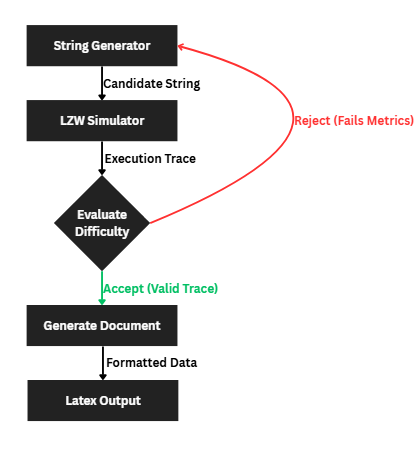
\includegraphics[width=0.85\linewidth]{images/architecture.png}
\caption{Data flow between the four components of the generation system. The string generator and difficulty evaluator together implement the difficulty control loop: candidates are generated and evaluated until one falls within the target band, or the attempt limit is reached.}
\label{fig:architecture}
\end{figure}

\section{Exercise Format Design}

A key design principle throughout this project is that a generated exercise should feel familiar to an appropriately prepared student. An exercise that requires students to learn a new notation or table format before attempting it wastes time in an examination setting and introduces a source of error unrelated to their understanding of the algorithm. The exercise format was therefore designed to match as closely as possible the examples used in the COMPSCI2026 algorithms course lecture slides.

\subsection{Correspondence with Lecture Material}

The step table used in the generated exercises reproduces the exact column structure from the class examples, as shown in Figure~\ref{fig:lectureexample}. The columns are: step number, position in the bitstream, the previous match, the binary code emitted or read, the output string, the new dictionary entry, and the assigned code index. A student who is appropriately prepared will recognise this layout immediately and can focus on applying the algorithm rather than interpreting the table structure.

\begin{figure}[htb]
\centering
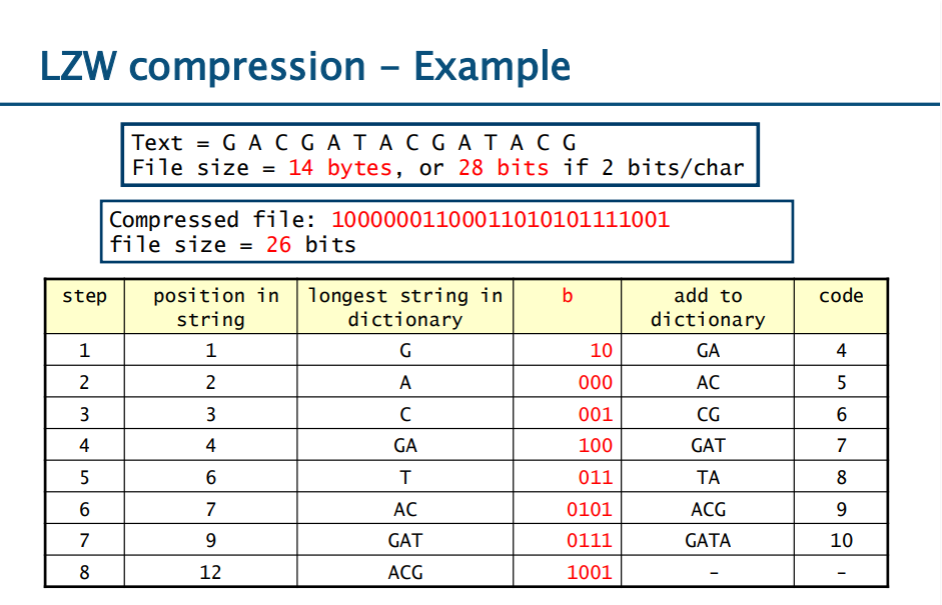
\includegraphics[width=0.85\linewidth]{images/lecture_example.png}
\caption{An example LZW step table from the COMPSCI2026 algorithms lecture slides. The generated exercises reproduce this column structure exactly.}
\label{fig:lectureexample}
\end{figure}

The choice of alphabet is similarly grounded in the lecture material. The four-symbol alphabet \{A, C, G, T\}, is the alphabet used in the class examples, and the initial dictionary assigns two-bit codes in the same order: A = 00, C = 01, G = 10, T = 11. Using this alphabet has two practical advantages beyond familiarity. With exactly four symbols, the initial dictionary fits neatly into two-bit codes, making the variable-width encoding easy to follow by hand. The alphabet is also small enough that the dictionary does not grow so large as to make the exercise unmanageable, but large enough that interesting multi-character matches arise within a tractable string length.

\subsection{The First-Row Scaffold}

One deliberate usability feature of the question sheet is that the first row of the step table is always completed for the student. There are two reasons for this. First, it disambiguates the table format: even if a student is uncertain how a column should be filled in, the worked first row provides a concrete reference. This is particularly important for the binary encoding column, where the variable bit width can be a source of confusion. Second, it reduces the effect of a student making an error on the very first step and then continuing that error for the remainder of the question. By anchoring the table, the exercise better isolates each student's understanding of the algorithm's main loop from their ability to initialise the procedure correctly.

\subsection{Concealing the Step Count}

A subtler design decision concerns how many blank rows to include in the question sheet. A naive implementation would include exactly as many blank rows as there are steps in the correct solution, which would inadvertently reveal the answer as a student who counts the blank rows would know exactly how many lines are rquired to complete the question. The design therefore adds a small number of extra blank rows beyond the true step count. Students therefore cannot then infer the number of steps from the table size, and must instead work through the algorithm until it terminates naturally.

\section{Difficulty Control}

\subsection{The Generation Loop}

The core design challenge is that an LZW exercise’s difficulty cannot be determined without first simulating the algorithm on the candidate string. There is no simple formula linking a string’s surface properties to its step count or dictionary growth. The design therefore adopts a \emph{generate-and-filter} approach, consistent with the strategy used by \citet{Hoz21} for SAT problems, strings are generated randomly and are accepted or rejected according to set structural constraints; each string must contain all four alphabet symbols, must not contain long runs of identical characters, and must produce a step count and dictionary size within the target band simulated.

This loop is shown in Algorithm~\ref{alg:genloop}.

\begin{algorithm}
\DontPrintSemicolon
\KwData{Target length $n$, difficulty profile $d$, attempt limit $M$}
\KwResult{A valid exercise trace, or failure}
\Begin{
    $i \longleftarrow 0$\;
    \While{$i < M$}{
        $s \longleftarrow \textsc{GenerateCandidate}(n, d)$\;
        \If{\textsc{HasIdenticalRun}$(s)$}{
            $i \longleftarrow i + 1$\;
            \textbf{continue}\;
        }
        $\text{trace} \longleftarrow \textsc{SimulateLZW}(s)$\;
        \If{\textsc{MeetsTargets}$(\text{trace}, n, d)$}{
            \Return trace\;
        }
        $i \longleftarrow i + 1$\;
    }
    \Return failure\;
}
\caption{The generate-and-filter loop for exercise generation.}
\label{alg:genloop}
\end{algorithm}

The attempt limit $M$ is a practical safeguard against the failure mode identified by \citet{Hoz21}: overly tight constraints can cause the generator to run indefinitely. By setting $M$ to a large but finite value, the system can report failure cleanly instead of hanging.

\subsection{Difficulty Profiles}

Two difficulty profiles are supported: high entropy and low entropy. These correspond to different target distributions for the input string and different expected execution behaviours, summarised in Table~\ref{tab:profiles}.

\begin{table}[htb]
\caption{Target properties of the two difficulty profiles. Step count targets are computed as a function of string length $n$; dictionary size targets combine a fixed base with a length-scaled growth term.}
\label{tab:profiles}
\rowcolors{2}{}{gray!3}
\begin{tabular}{@{}lll@{}}
\textbf{Property} & \textbf{High Entropy} & \textbf{Low Entropy} \\ Character distribution & Approximately uniform & Skewed toward one symbol \\ Target step count & $\approx 0.65n$ & $\approx 0.65n$ \\ Dictionary growth scaling & $0.7n$ above base & $0.4n$ above base \\ Max consecutive identical chars & 2 & 3 \\
\end{tabular}
\end{table}

The target step count is kept constant across profiles so that both generate exercises requiring the same amount of written work. What differs is the nature of that work: high-entropy exercises require students to track unpredictable sequences, whereas low-entropy exercises involve recognising repeated patterns. This distinction is reflected partly in Shannon entropy and partly in the variance of the input.

\subsection{Shannon Entropy as a Difficulty Signal}

Shannon entropy is computed from the character frequency distribution of the input string, as defined in Chapter~2. For the four-symbol alphabet \{A, C, G, T\}, maximum entropy is $\log_2 4 = 2$ bits per symbol, achieved when all four characters appear with equal frequency. Low-entropy strings have a dominant character whose frequency pulls the distribution away from uniform.

Entropy is used in this design as a diagnostic metric rather than a primary filter. As \citet{KosarajuManzini99} show, the relationship between entropy and LZW execution behaviour is not tight for short strings: two strings with similar entropy can produce very different step counts. The primary difficulty controls are therefore step count and dictionary growth, with entropy reported alongside each exercise in the terminal output to allow an educator to check consistency across a batch.

\subsection{Input Variance}

Input variance is an additional difficulty signal not captured by Shannon entropy. A student tracing the LZW algorithm by hand is affected not only by the statistical regularity of the string but also by its appearance. A string such as \texttt{AAACAAAC} contains obvious visual structure that a student will recognise and use to form expectations about the execution. A string such as \texttt{ACGTCAGT} appears irregular, requiring the student to engage with each step independently.

Input variance is measured as the number of distinct adjacent character pairs (bigrams) in the input string, normalised by the maximum possible number of distinct bigrams given the alphabet size. Formally, for a string $s$ of length $n$ over alphabet $\Sigma$:

\begin{equation}
    V(s) = \frac{|\{(s_i, s_{i+1}) : 1 \leq i < n\}|}{|\Sigma|^2}
\end{equation}

A string with high input variance has many distinct adjacent pairs, appearing irregular to a reader. A string with low input variance has few distinct pairs, appearing patterned. This measure is simple to compute and is independent of entropy: a low-entropy string can have either high or low input variance depending on whether the dominant character appears in varied contexts.

Input variance is introduced in this project as a novel difficulty signal for LZW exercises. No known prior work on automated exercise generation, including \citet{Hoz21} and \citet{PriorGlasgow}, identifies the visual appearance of the input string as a dimension of perceived difficulty distinct from its statistical properties. The observation that motivates it is straightforward: two strings with identical Shannon entropy can look very different to a student reading them, and that difference in appearance affects how easily a student can form expectations about the execution before they begin tracing. Bigram diversity was chosen because it is the simplest measure that captures adjacency structure rather than just character frequency, requires no algorithm simulation, and produces a continuous value that varies independently of entropy across the generated string space.

\section{LZW Simulation Design}

\subsection{Compression}

The compression simulator processes the input string left to right, maintaining a dictionary initialised with the four base symbols. At each step it extends the current match as far as possible, then emits the binary code for the match using a variable bit width determined by the current dictionary size:

\begin{equation}
    \text{bit width} = \lceil \log_2(\text{dict size}) \rceil
\end{equation}

Students must track not only the dictionary entries but also the number of bits used at each step. The simulator records the position in the bitstream where each code begins, so that the question sheet can show students where to start reading at each step.

The final symbol in the input is always emitted using the dictionary size after all preceding entries have been added, because no new entry is created at the last step. This edge case is handled explicitly in the simulator and is reflected in the answer key, where the last row leaves the “string added” column empty.

\subsection{Decompression}

The decompression simulator takes the binary stream produced by compression and reconstructs the step-by-step trace. It reads bits from the stream using the same variable-width rule, looks up each code in the incrementally rebuilt dictionary, and reconstructs the original string. The standard decompression edge case, where a code is encountered before its dictionary entry is fully defined, is handled by the well-known rule that the new string is the previous output concatenated with its own first character. The simulator detects and resolves this case, and the answer key marks the affected row distinctively so that educators can identify it as a teaching point. The generator can optionally target this case directly: a detection function checks whether any step in the simulated trace emits a code equal to the current dictionary size at the moment of emission, which is the condition that triggers the edge case during decompression. When the special case mode is enabled, candidate strings that do not trigger this condition are rejected before their trace is accepted.

\subsection{Trace Format}

Both simulators produce traces in the same tabular format, which maps directly onto the step table presented to students. Each row contains the step number, the bit position in the file, the previous match, the binary code, the output string, the new dictionary entry, and the assigned code index. The document generator consumes this format without modification, ensuring that the answer key is always consistent with the simulated execution.

\section{Document Generation Design}

\subsection{Output Format}

The document generator produces output in LaTeX format. This was decided with the lecturer who would be using the tool: LaTeX integrates directly into the existing means for producing course materials and examination papers at the University of Glasgow. Producing LaTeX source rather than a PDF directly gives the educator full control over final formatting, allows exercises to be embedded within a larger examination document, and makes it straightforward to adjust spacing or typography without regenerating the exercise.

\subsection{Question and Answer Sheet Structure}

Each generated exercise produces two documents with identical structure but different content. Both begin with a header showing the input sequence (for compression) or compressed bitstream (for decompression), the initial dictionary, and the task instructions. Both contain the step table with the same column headers.

In the question sheet, only the first row of the step table is populated, as a worked example as described in Section~4.2.2. Additional blank rows beyond the true step count are included to conceal the answer, as described in Section~4.2.3. In the answer key, all rows are populated and rows containing multi-character matches are visually distinguished, since these are the steps where students most commonly make errors.

\subsection{Batch Output and Metrics Logging}

When generating a batch of exercises, the system produces separate question and answer files for each exercise, organised into distinct output folders. The generator prints the key difficulty metrics for each exercise to the terminal, giving the educator immediate confirmation of the properties of each generated question.

\section{User Interface Design}

The system is operated through a minimal command-line interface rather than a graphical application. This is a deliberate design decision. The target user is an educator who will run the generator occasionally to produce a batch of exercises; a graphical interface would add significant implementation complexity without providing meaningful benefit for this use case.

The interface presents the user with a small number of clearly labelled choices: a  string length between 8 and 30 characters, a choice between high and low entropy profile, and a count of how many exercises to generate. Default values are provided for all parameters so that the tool can be run immediately without configuration. The educator's concern is the difficulty level and quantity of exercises, not the internal parameters of the generation algorithm, so exposing only these three controls keeps the interface accessible without requiring deep knowledge of how the generator works.


%==================================================================================================================================
\chapter{Implementation}

This chapter describes the implementation of the LZW exercise generation system. The system is written in Python and consists of two independent scripts: one for compression exercises and one for decompression exercises. Both follow the architecture described in Chapter~4. The chapter covers the key implementation decisions in each component, with particular attention to aspects where the implementation required non-trivial solutions.

\section{Overview}

The system consists of two Python scripts: one for compression exercises and one for decompression exercises. Both follow the four-component architecture described in Chapter~4 and share the same core logic for string generation, LZW simulation, and difficulty. Python was chosen because its standard library covers everything needed; string processing, random sampling, and maths without requiring any external dependencies.

The compression generator takes a string length, difficulty profile, and batch size as input, then produces LaTeX question and answer sheets. The decompression generator works the same way but additionally asks whether the generated exercises should include the special case, where a code is encountered before its dictionary entry is fully defined.

Both generators produce output in the same folder structure: question sheets in \texttt{Questions/} and answer keys in \texttt{Answers/}.

\section{String Generation and Difficulty Control}

\subsection{The Generate-and-Filter Loop}

The main implementation challenge is generating strings whose LZW execution falls within a desired range. As there is no closed-form relationship between a string's characters and its step count or dictionary growth, the approach taken is to generate candidates and reject those that do not meet the targets.

The generator creates each candidate by first drawing all four symbols without replacement, guaranteeing that every generated string contains at least one occurrence of each character in the alphabet. This prevents bad cases where a symbol is absent entirely, which would reduce the effective alphabet size and break the assumption that the initial dictionary has four entries. The remaining characters are drawn with profile-dependent weights: uniform (0.25 each) for high entropy, and skewed (0.65, 0.18, 0.10, 0.07) for low entropy. The string is then shuffled to remove any ordering bias introduced by the sampling procedure.

\begin{lstlisting}[language=Python, float,
  caption={The candidate string generation procedure. All four symbols are
  guaranteed to appear by seeding with a permutation of the alphabet before
  drawing the remaining characters with profile-dependent weights.},
  label=lst:gencandidate]
text_list = random.sample(SYMBOLS, len(SYMBOLS))
text_list += random.choices(SYMBOLS, weights=weights, k=length - 4)
random.shuffle(text_list)
text = "".join(text_list)
\end{lstlisting}

Before simulation, each candidate is tested for long runs of identical characters. A string is rejected if it contains more than \texttt{max\_streak} consecutive identical symbols, where \texttt{max\_streak} is 2 for high entropy and 3 for low entropy. Strings with long runs produce exercises where many consecutive steps are trivially identical, reducing their value as assessment questions regardless of their formal entropy.

After passing the streak test, the string is simulated using \texttt{simulate\_lzw}, which returns the final dictionary size and the list of output codes. A candidate is accepted if its step count and dictionary size are both within one of their respective targets, and if the compressed output is strictly shorter than the original string in symbols. To avoid the generator hanging on difficult parameter combinations, the acceptance tolerance is widened slightly every 25,000 attempts. If no candidate is accepted within 100,000 iterations, the loop exits and returns the most recent result as a best-effort fallback.

\subsection{Target Computation}

The step count target is computed as $\lfloor 0.65n \rfloor$, floored at 4, where $n$ is the string length. This formula was derived empirically: it produces a number of steps that is tractable for a student to complete in an examination setting while still requiring a meaningful trace of the algorithm. The dictionary size target combines a fixed base of four entries with a profile-dependent linear growth term:

\begin{equation}
    D_{\text{target}}(n, p) = 4 + \max\!\left(3,\ \lfloor n \cdot s_p \rfloor\right),
\end{equation}

where $s_p$ is the scaling factor for profile $p$: 0.7 for high entropy and 0.4 for low entropy. The higher scaling factor for high entropy reflects that uniform character distributions produce more distinct substrings and therefore more dictionary entries per unit of input length.

Figure~\ref{fig:steps_vs_length} shows that both profiles track the target step count closely across the full range of supported string lengths, with the shaded standard deviation bands collapsing almost to zero. The high entropy profile produces systematically more steps than low entropy at the same length, a consequence of its larger dictionary target requiring the algorithm to build more entries before revisiting matches.

\begin{figure}[htb]
    \centering
    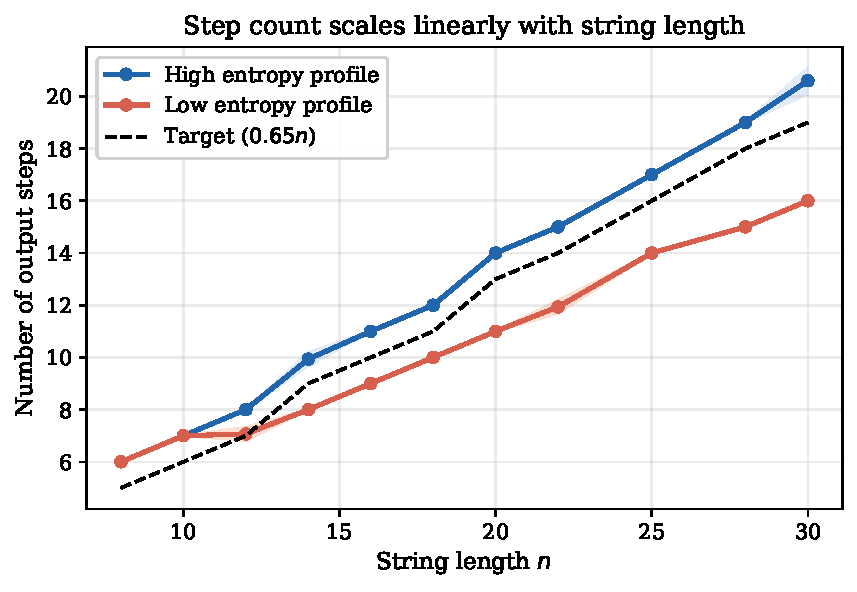
\includegraphics[width=0.85\linewidth]{images/figures/fig1_steps_vs_length.pdf}
    \caption{Mean step count (with $\pm 1$ standard deviation shading) for 15 generated exercises per profile at each string length. Both profiles track the target $0.65n$ line closely. The high entropy profile produces more steps than low entropy at the same length because its larger dictionary target requires more distinct matches before the algorithm begins reusing entries.}
    \label{fig:steps_vs_length}
\end{figure}

\section{LZW Simulation}

\subsection{Compression}

The compression simulator starts with a dictionary containing the four base symbols and reads the input from left to right, always trying to extend the current match as far as possible. When adding the next character would go beyond a known dictionary entry, the simulator outputs the current match as a code, adds the new entry to the dictionary, and starts the match again from that character. The number of bits used to encode each code is calculated at that moment as $\lceil \log_2(\text{dict size}) \rceil$, where dict size counts the entries before adding the new one. This is the same approach used in the lecture slides and ensures the decoder can reconstruct the correct bit widths from the dictionary alone.

An important edge case is the final symbol of the input, which is always emitted even though it does not trigger the addition of a new dictionary entry. The implementation handles this by appending a final step after the main loop exits, using the current dictionary size at that point. In the answer key, this final row has a dash in both the ``String Added'' and ``Code Created'' columns, as shown in the bottom row of Figure~\ref{fig:compression_answer}.

\subsection{Decompression}

The decompression simulator operates on the binary stream produced by compression. At each step it reads the appropriate number of bits, looks up the code in the incrementally rebuilt dictionary, and outputs the corresponding string. The bit width at each step is computed using the same formula as compression, applied to the decoder's current dictionary size, which mirrors the encoder's state because both process the same sequence of codes.

The standard decompression special case arises when a code is encountered that has not yet been added to the decoder's dictionary. This occurs when the encoder emits a code for a string that was only just added in the previous step. The decoder handles this by constructing the missing entry as the previous output string concatenated with its own first character. This case is noted in the answer key through the Special Case: Yes field reported in the terminal output, allowing an educator to identify which exercises contain it before distributing papers.

There is also an optional mode that guarantees the special case appears in every generated exercise. The way this works is that each candidate string is run through a detection function, \texttt{has\_special\_case}, which checks whether any emitted code during compression equals \texttt{dict\_size - 1} at the moment it is output — the exact condition that will trip up the decoder. Strings that do not trigger this are rejected and the generator tries again. This lets an educator decide whether they want to specifically test the edge case or leave it out entirely for students who are still getting to grips with the basic algorithm.

\section{Document Generation}

\subsection{Compression: LaTeX Output}

The compression document generator produces two LaTeX files per exercise: a question sheet and an answer key. Both are standalone LaTeX documents that can be compiled directly or embedded within a larger examination paper.

Figure~\ref{fig:terminal_output} shows the terminal output when generating a batch of compression exercises. The generator reports the input string, Shannon entropy, input variance, step count, dictionary size, and the paths to the generated files for each question. This gives an educator immediate confirmation of the difficulty properties of each exercise without needing to open the generated files.

\begin{figure}[htb]
    \centering
    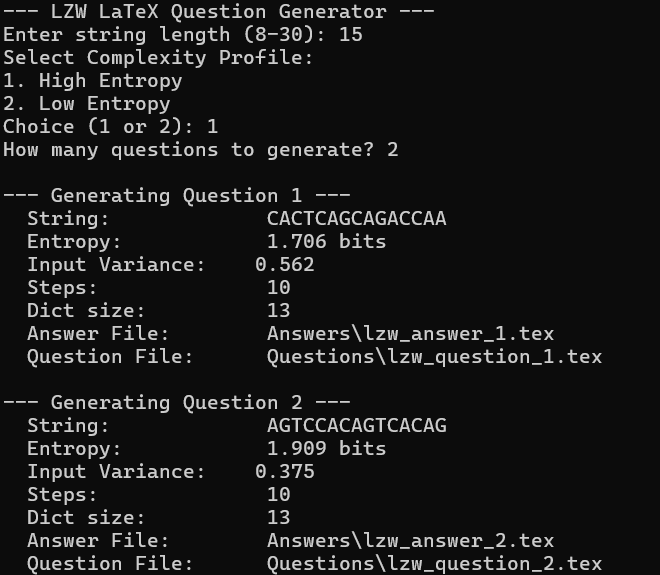
\includegraphics[width=\linewidth]{images/terminal_output.png}
    \caption{Terminal output when generating a batch of compression exercises. Each question is reported with its key difficulty metrics alongside the paths to the generated question and answer files.}
    \label{fig:terminal_output}
\end{figure}
\clearpage
\begin{figure}[htb]
    \centering
    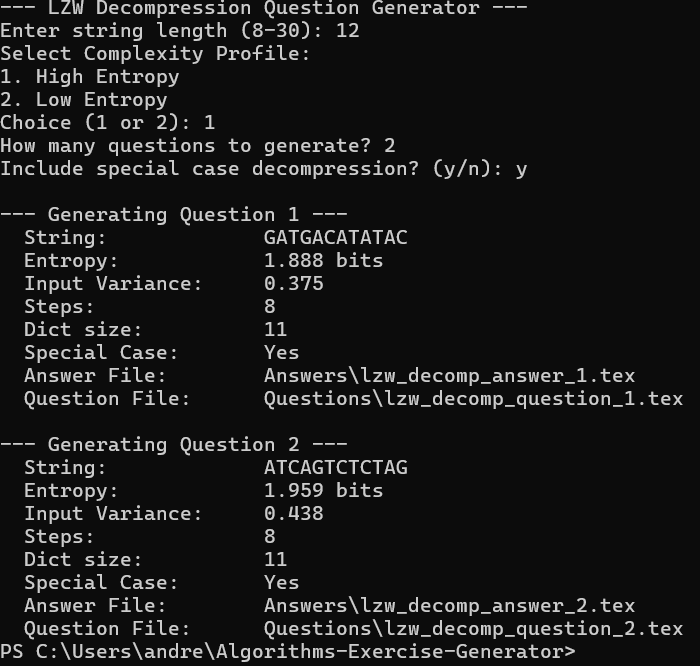
\includegraphics[width=\linewidth]{images/terminal_output_specialcase.png}
    \caption{Terminal output when generating decompression exercises with special case mode enabled. The Special Case: Yes field confirms that the generated exercise contains the LZW decompression edge case, where a code is encountered before its dictionary entry is fully defined. This allows an educator to specifically target this aspect of the algorithm for assessment.} \label{fig:terminal_output_specialcase}
\end{figure}

The question sheet, shown in Figure~\ref{fig:compression_question}, displays the input sequence in a per-character table at the top of the page, followed by the task instructions and the step table. The first row of the step table is pre-populated with the correct values for step 1, providing a worked example that anchors the table format for the student. All remaining rows are blank. The number of blank rows is equal to the true step count plus four additional rows, so that the table size does not reveal the answer to the student.

The answer key, shown in Figure~\ref{fig:compression_answer}, uses the same layout but populates all rows with the correct values from the simulation trace. The header is marked ``Examiner Solution Key'' to distinguish it from the student's question sheet.

\begin{figure}[htbp]
    \centering
    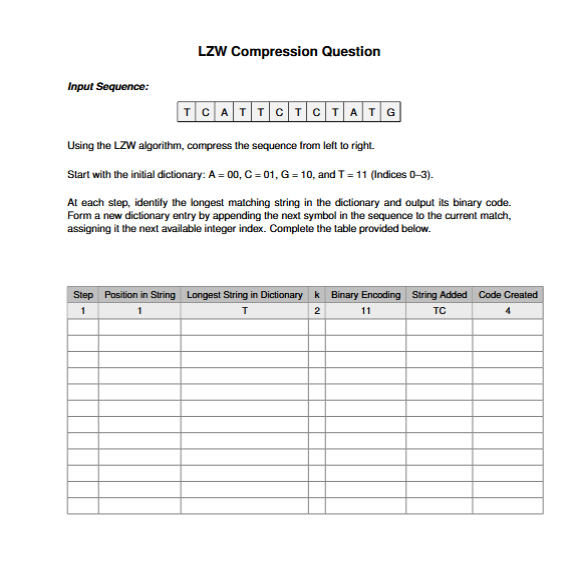
\includegraphics[width=0.7\linewidth]{images/compression_question.png}
    \caption{Student question sheet. Only step~1 is completed; the remaining rows are blank. Four additional rows beyond the true step count conceal the answer length.}
    \label{fig:compression_question}
\end{figure}

\begin{figure}[htbp]
    \centering
    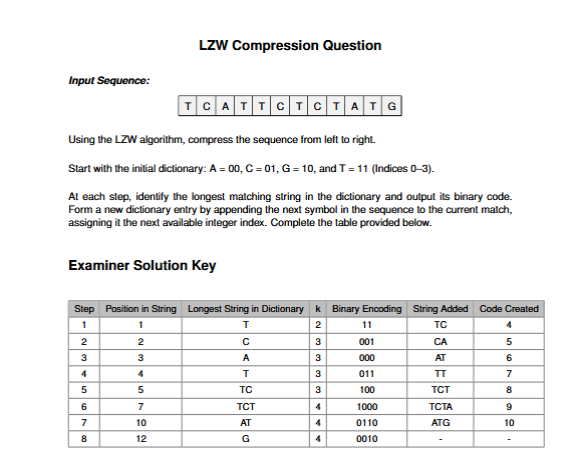
\includegraphics[width=0.7\linewidth]{images/compression_answer.png}
    \caption{Examiner answer key for the same exercise. All ten steps are populated. The final row has dashes in the last two columns because no new dictionary entry is created at the final step.}
    \label{fig:compression_answer}
\end{figure}
\newpage
\subsection{Decompression: LaTeX Output}

The decompression generator produces LaTeX output for each exercise using the same formatting approach as the compression generator. Column headers are shaded using \texttt{xcolor}, the worked example row is given a grey background to distinguish it from the student-completed rows, and extra blank rows are added beyond the true step count to conceal the answer length.

The decompression question sheet gives students the compressed bitstream and the file size in bits, with the uncompressed text field left blank for them to fill in. The answer key populates the uncompressed text field and all table rows, as shown in Figure~\ref{fig:decompression_answer}.

\begin{figure}[htb]
    \centering
    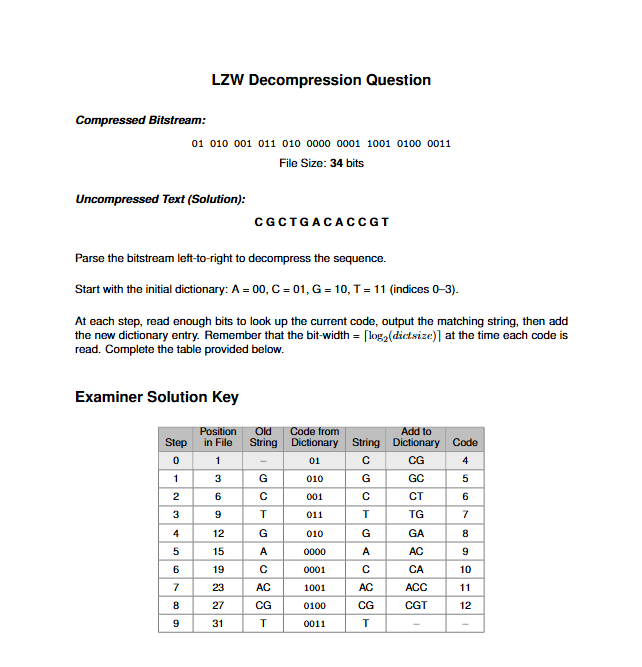
\includegraphics[width=1\linewidth]{images/decompression_answer.png}
    \caption{Generated decompression exercise answer key.}
    \label{fig:decompression_answer}
\end{figure}
\clearpage


\section{Scaling Behaviour}

Figure~\ref{fig:entropy_vs_length} shows that Shannon entropy stabilises quickly with string length and remains well-separated between profiles from $n = 8$ upwards. The high entropy profile consistently achieves values near the theoretical maximum of 2 bits per symbol; the low entropy profile stabilises around 1.5 bits. The standard deviation bands widen slightly at shorter lengths, reflecting that character frequency distributions are more variable in very short strings.

\begin{figure}[htb]
    \centering
    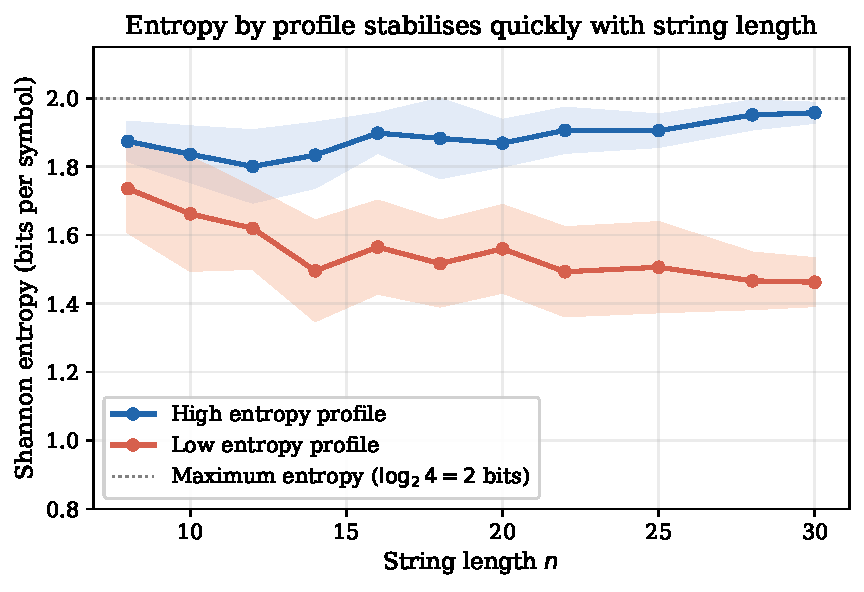
\includegraphics[width=0.85\linewidth]{images/figures/fig2_entropy_vs_length.pdf}
    \caption{Mean Shannon entropy with $\pm 1$ standard deviation shading across 15 exercises per profile. Entropy stabilises from $n \approx 10$ onward and remains well-separated between profiles. The dotted line marks the theoretical maximum of $\log_2 4 = 2$ bits per symbol.}
    \label{fig:entropy_vs_length}
\end{figure}

Figure~\ref{fig:dictsize_vs_length} shows dictionary growth for both profiles. The high entropy profile grows faster, consistent with its larger target scaling factor (0.7 versus 0.4). The dashed target lines track the observed means closely. At longer lengths, the actual dictionary sizes begin to slightly undercut their targets, which reflects the widening of the acceptance tolerance at longer lengths described in Section~5.2.1.

\begin{figure}[htb]
    \centering
    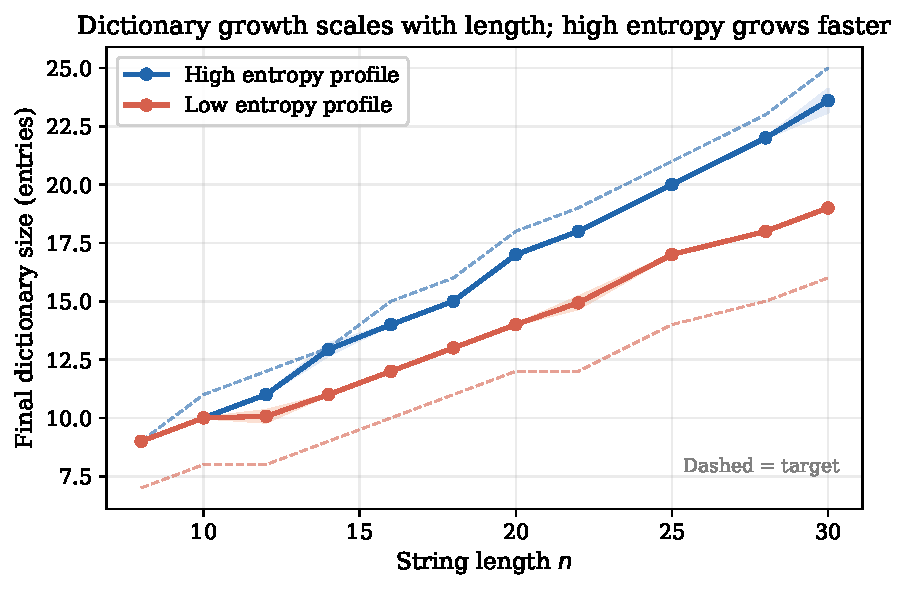
\includegraphics[width=0.85\linewidth]{images/figures/fig3_dictsize_vs_length.pdf}
    \caption{Mean final dictionary size with $\pm 1$ standard deviation shading. Dashed lines show the computed target for each profile. High entropy strings grow the dictionary faster due to their larger scaling factor (0.7 vs 0.4) producing exercises where the bit width increases more frequently over the course of the trace.}
    \label{fig:dictsize_vs_length}
\end{figure}

Figure~\ref{fig:attempts_vs_length} shows an difference between the two profiles that is not visible from the output metrics alone. The low entropy profile requires consistently around 10,000 to 20,000 generation attempts at all string lengths, while the high entropy profile requires far fewer at moderate lengths but spikes at $n = 30$. Low entropy strings are structurally harder to satisfy simultaneously for both step count and dictionary size, because their skewed character distribution tends to produce fewer distinct substrings, making the dictionary grow more slowly and step counts harder to hit. The spike for high entropy at $n = 30$ occurs because the combined tolerance on both targets becomes difficult to satisfy with strictly uniform character weights at longer lengths.

\begin{figure}[htb]
    \centering
    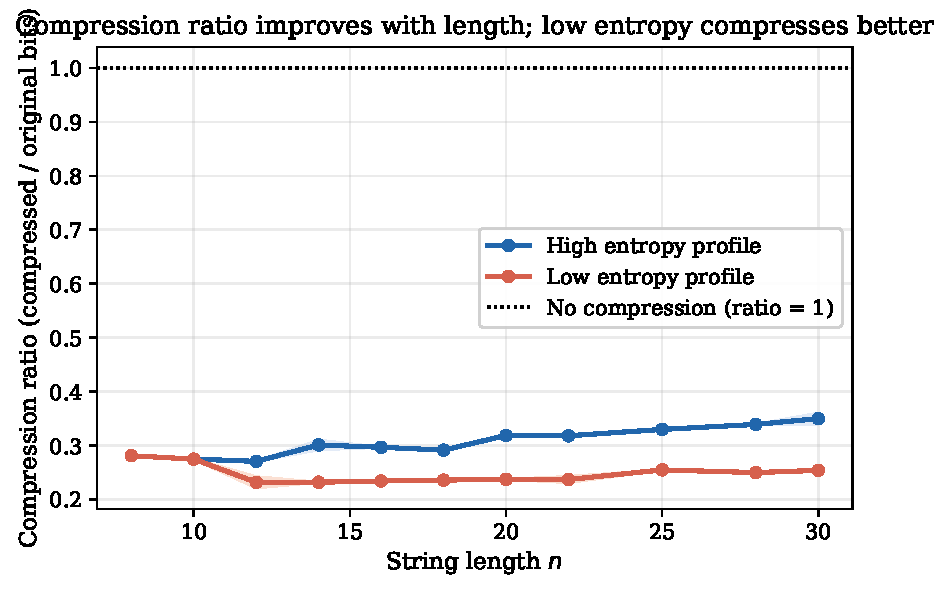
\includegraphics[width=0.85\linewidth]{images/figures/fig4_ratio_vs_length.pdf}
    \caption{Mean generator attempts required before a valid string is accepted (log scale, $\pm 1$ standard deviation shading). The low entropy profile requires consistently high attempt counts at all lengths. The spike for high entropy at $n = 30$ reflects increasing difficulty satisfying both constraints simultaneously at longer lengths with strictly uniform weights.}
    \label{fig:attempts_vs_length}
\end{figure}
 
The 100,000-attempt limit is generous enough to succeed reliably at all tested lengths, but an educator choosing string lengths above 25 with the low entropy profile should expect marginally longer generation times. The attempt count data also validates the decision to use a finite attempt limit: without it, corner cases at the extremes of the supported length range could cause the generator to hang indefinitely, as was observed during development.


%==================================================================================================================================
\chapter{Evaluation}

This chapter evaluates the system against the requirements established in
Chapter~3. Three questions structure the evaluation:

\begin{enumerate}
    \item Does the generator produce exercises of consistent and controllable
    difficulty?
    \item Do students experience the generated exercises as fair, clear, and comparable to exercises they encounter in class?
    \item Is the system usable by someone generating exercises for a class test?
\end{enumerate}

The first question is addressed through quantitative analysis of generated exercise properties. The second is addressed through a class test study with COMPSCI2026 algorithms students. The third is addressed through a usability study with participants who interacted directly with the generator.

\section{Difficulty Consistency}

\subsection{Step Count Control}

The most direct measure of whether exercises are equally difficult is step count, since each step corresponds to one row the student must complete in the table. Figure~\ref{fig:steps_vs_length} shows that both profiles track the $0.65n$ target closely across all tested lengths, with standard deviation that is almost 0, so within a batch generated for a fixed length and profile, every exercise requires almost the same number of steps.

Table~\ref{tab:consistency} summarises the consistency metrics for a batch of 60 exercises generated at $n = 15$ for each profile.The coefficient of variation (CV) measures how spread out the values are relative to the mean as a lower CV means the difficulty is more consistent.

\begin{table}[htb]
\caption{Difficulty consistency metrics for 60 generated exercises per profile at string length $n = 15$. CV denotes coefficient of variation (standard deviation / mean $\times$ 100\%).}
\label{tab:consistency}
\rowcolors{2}{}{gray!3}
\begin{tabular}{@{}llllll@{}}
\textbf{Metric} & \textbf{Profile} & \textbf{Mean} & \textbf{Std dev}
    & \textbf{Min} & \textbf{Max} \\
Step count      & High entropy & \num{10.00} & \num{0.00} & 10 & 10 \\
Step count      & Low entropy  & \num{8.00}  & \num{0.00} & 8  & 8  \\
Shannon entropy & High entropy & \num{1.85}  & \num{0.11} & \num{1.53} & \num{1.99} \\
Shannon entropy & Low entropy  & \num{1.50}  & \num{0.13} & \num{1.38} & \num{1.75} \\
Dictionary size & High entropy & \num{14.57} & \num{0.50} & 14 & 15 \\
Dictionary size & Low entropy  & \num{10.10} & \num{0.30} & 10 & 11 \\
\end{tabular}
\end{table}

Step count CV is 0\% for both profiles at $n = 15$, confirming that the acceptance criteria is functioning as intended. Shannon entropy varies more, with a standard deviation of approximately 0.11 bits for high entropy and 0.13 bits for low entropy. This is expected: the generator controls step count and dictionary size directly and treats entropy as a diagnostic signal. The entropy variation reflects the natural diversity of strings that satisfy the step count and dictionary constraints.

\subsection{Entropy and Input Variance}

Figure~\ref{fig:entropy_vs_vv_eval} shows the relationship between Shannon entropy and input variance across all generated exercises. The two metrics are correlated within each profile, but the relationship is not tight. Two exercises with similar entropy values can differ substantially in input variance, and therefore in the perceptual difficulty a student experiences when reading the input before beginning to trace the algorithm. This confirms the design claim from Section~4.3.4 that entropy alone does not fully determine how patterned a string appears to a student.

\begin{figure}[htb]
    \centering
    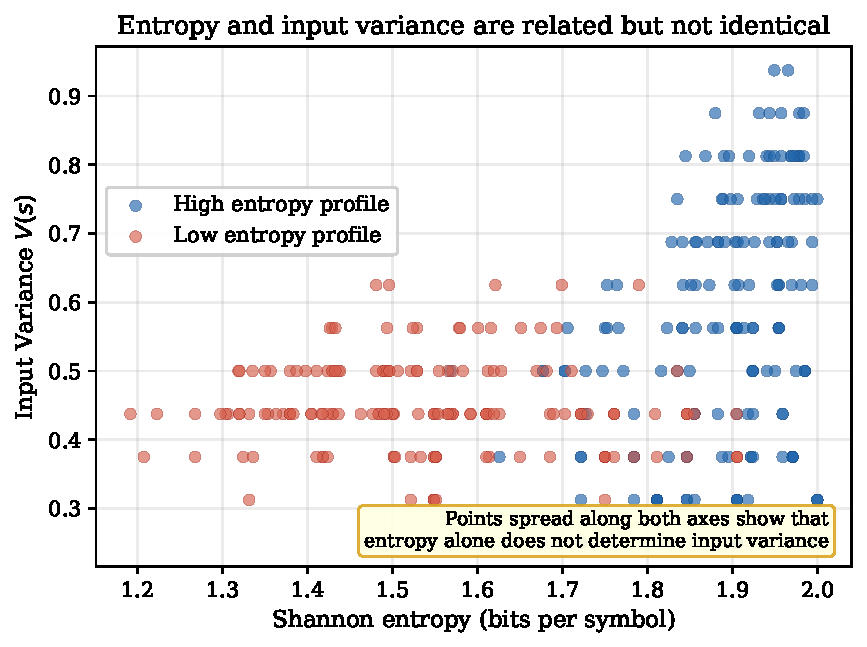
\includegraphics[width=0.85\linewidth]{images/figures/fig5_entropy_vs_iv.pdf}
    \caption{Shannon entropy versus input variance $V(s)$ for all generated
    exercises across all tested string lengths. Points are coloured by
    difficulty profile. The spread along both axes within each profile
    confirms that entropy and input variance are related but not identical,
    justifying the use of both metrics in the difficulty framework.}
    \label{fig:entropy_vs_vv_eval}
\end{figure}

\newpage

\section{Class Test Study}

Five students enrolled in COMPSCI2026 completed a generated LZW compression or decompression exercise under test-like conditions, then filled in a short questionnaire about their experience. All participants provided informed consent prior to taking part, and the study was conducted in accordance with the School of Computing Science ethics checklist, a signed copy of which is included in Appendix~A. All five reported feeling Confident or Very Confident in their understanding of LZW, which is a useful baseline as feedback from students who already knew the material is more meaningful than feedback from those still learning it.

\begin{table}[htb]
\label{tab:class_test_summary}
\rowcolors{2}{}{gray!3}
\begin{tabular}{@{}lll@{}}
\textbf{Question} & \textbf{Positive} & \textbf{Other} \\
Confidence in LZW              & 5/5 (100\%) & 0 \\
Similarity to class examples   & 4/5 (80\%)  & 1 neutral \\
Tested understanding           & 5/5 (100\%) & 0 \\
Clarity of generated input     & 5/5 (100\%) & 0 \\
Fairness of differentiation    & 2/5 (40\%)  & 1 neutral, 2 negative \\
\end{tabular}
\caption{Summary of class test study responses ($n = 5$). Positive responses
are those in the top two categories for each question.}
\end{table}

The results for the first four questions were positive. 80\% of participants rated the generated questions as similar or very similar in difficulty to questions they had seen in class, with the remaining 20\% selecting neither similar nor dissimilar. All five agreed or strongly agreed that the question tested their understanding of LZW principles, and all five found the randomly generated input string clear or very clear to work with.

The fairness question produced the most mixed responses. Two participants strongly agreed that receiving different but equally difficult questions is fair, one was neutral, one disagreed, and one strongly disagreed. The free-text responses suggest the split comes down to a distinction between varying the input string, which participants were broadly comfortable with, and varying the type of question or algorithm, which they were not. This is consistent with how the generator works: every student gets a different string but the same question type, algorithm, and table format. The negative responses likely reflect a general discomfort with differentiated assessments rather than a specific dislike to this approach. Given the sample size of five, these results should be treated as indicative rather than conclusive.

\section{Usability Study}

Eleven participants with a computing science background were given access to the compression and decompression question generators. All participants provided informed consent prior to taking part under the same ethics approval. They were free to use the generators as much as they wished before completing a short survey evaluating both usability and output quality.

Overall, responses were consistently positive. All participants rated the generator interface as intuitive or very intuitive, and all trusted the generator to produce fair questions. Ten out of eleven participants felt that questions with different symbol patterns varied in difficulty, even when requiring the same number of steps (the remaining participant selected maybe rather than no). In addition, all participants agreed or strongly agreed that step count scales proportionally with string length, supporting the  results shown in Figure~\ref{fig:steps_vs_length}.

The most useful insight came from Questions 4 and 5. All eleven participants found low-entropy, repetitive-pattern questions easier than high-entropy, more evenly distributed ones, with seven choosing slightly easier and four choosing much easier. No one thought they were equally difficult or harder. This supports the idea behind the two-profile design: difficulty isn’t just about the number of steps. The way characters are distributed in the input also has a clear impact on how hard a question feels. This is exactly what input variation is trying to capture.

\begin{table}[htb]
\label{tab:usability_summary}
\rowcolors{2}{}{gray!3}
\begin{tabular}{@{}lll@{}}
\textbf{Question} & \textbf{Positive} & \textbf{Other} \\
Interface usability              & 11/11 (100\%) & 0 \\
Trust generator is fair          & 11/11 (100\%) & 0 \\
Symbol patterns feel different   & 10/11 (91\%)  & 1 maybe \\
Repetitive patterns feel easier  & 11/11 (100\%) & 0 \\
Input differences affect difficulty & 9/11 (82\%) & 2 neutral \\
Step count scales with length    & 11/11 (100\%) & 0 \\
\end{tabular}
\caption{Summary of usability study responses ($n = 11$). Positive responses are those in the top two categories for each question.}
\end{table}

Nine out of eleven participants agreed or strongly agreed that differences in automatically generated inputs can affect how difficult a question feels, while two selected neutral and none disagreed. This lines up with the results from Questions 4 and 5, suggesting that participants not only noticed but also experienced the impact of character distribution on difficulty, separate from the number of steps involved.

As this was a usability study rather than a controlled experiment, the findings should be interpreted as indicative rather than definitive. However, the consistency of responses provides  confidence that the question generator design and output functions as intended.

\section{Requirements Review}

Table~\ref{tab:requirements_review} summarises the extent to which each
must-have and should-have requirement from Chapter~3 was satisfied.

\begin{table}[htb]
\caption{Review of must-have and should-have requirements against the
evidence gathered in this chapter.}
\label{tab:requirements_review}
\rowcolors{2}{}{gray!3}
\begin{tabular}{@{}p{7cm}p{2cm}p{4cm}@{}}
\textbf{Requirement} & \textbf{Status} & \textbf{Evidence} \\
Generate valid LZW compression exercises in LaTeX & Met &
    Table~\ref{tab:consistency} \\
Generate valid LZW decompression exercises & Met &
    Figure~\ref{fig:decompression_answer} \\
Well-formedness: compression required, step count in range & Met &
    Table~\ref{tab:consistency}; Figure~\ref{fig:steps_vs_length} \\
Difficulty profile controls entropy and step count & Met &
    Table~\ref{tab:consistency} \\
Produce question sheet and answer key per exercise & Met &
    Table~\ref{tab:consistency} \\
Configurable batch size & Met & Section~5.2 \\
Metrics reported to terminal per exercise & Met & Figure~\ref{fig:terminal_output} \\
Reject strings with long identical-character runs & Met & Section~5.2.1 \\
Usable with three parameters or fewer & Met & Section~4.6 \\
Generator correctness: answer key matches simulation & Met &
    Design guarantees consistency by construction \\
Consistent difficulty within a batch (low step CV) & Met &
    CV = 0\% at $n=15$; Table~\ref{tab:consistency} \\
Graceful failure on no valid string found & Met & Section~5.2.1 \\
\end{tabular}
\end{table}


%==================================================================================================================================
\chapter{Conclusion}

\section{Summary}

This project set out to build a system that automatically generates LZW compression and decompression exercises for use in class tests, where the goal is for each student to receive a different question that is still equally difficult. To the best of my knowledge, no prior work has addressed automated exercise generation for data compression algorithms, despite LZW being a standard topic in undergraduate algorithms courses.

The motivation for this approach came straight from noticing the tension between fairness and collusion resistance in class tests. The key insight was that LZW’s step-by-step execution produces a structured, verifiable trace, which maps naturally onto a table exercise. Instead of trying to control difficulty through the input string itself, I realised it could be managed by targeting properties of that trace. This led to the generate-and-filter design: generate candidate strings, simulate the algorithm, and accept or reject them based on whether the execution falls within a desired difficulty band.

The outcome of this work is the development of two Python-based tools that generate fully formatted LaTeX question and answer sheets fit for use in class tests. Both compression and decompression exercises are supported, including the decompression special case where a code is encountered before its dictionary entry is fully defined. Difficulty is controlled through step count and dictionary size targeting, with Shannon entropy and input variance tracked as diagnostic measures. Across 60 generated exercises per profile at $n = 15$, step count coefficient of variation was 0\%, meaning every exercise in a batch required exactly the same number of written steps. The two profiles were well-separated on Shannon entropy (means of \num{1.85} and \num{1.50} bits per symbol), and all generated exercises compressed successfully. A class test study with five COMPSCI2026 students (drawn from a pool of 18) found that generated exercises were rated as comparable in difficulty to class examples, clear to work with, and effective at testing understanding of the algorithm.

\section{Reflection}

One insight that only became clear after running the generator at scale was just how many attempts the low-entropy profile requires — consistently between 10,000 and 20,000 per exercise. The tolerances and weight vectors were tuned through trial and error, which worked but involved a lot of iteration before the generator behaved reliably. Given more time, it would have been useful to analyse the distribution of LZW step counts for a given character weight vector beforehand, so the acceptance criteria could be set more precisely from the start rather than adjusted through repeated testing.

The compression and decompression generators were also developed somewhat independently, which led to duplicated logic and inconsistent quality criteria between the two. Extracting the shared difficulty control code into a common module from the start would have made the system easier to maintain and extend.

Finally, input variance is controlled indirectly through the character weight choices for each profile, which were tuned to produce strings that feel appropriately varied or patterned. However, this is fixed at design time rather than being something an educator can adjust. In hindsight it would have been better to use input variance as a parameter, so that an educator could request strings that appear more or less visually regular independently of the entropy profile.

\section{Future Work}

\paragraph{Interface and student use.} 
The command-line interface is currently aimed at educators producing exercise batches. A simple web interface could make it easier for them to configure and download exercises without using a terminal. The generator could also serve as a student practice tool, enabling unlimited attempts before a test and supporting self-study with verified, automatically generated questions.

\paragraph{Additional algorithms.}
The most direct extension would be to add support for Huffman coding. Like LZW, Huffman coding has a step-by-step execution that translates naturally into a table exercise, and its difficulty is tied to character frequencies in a way that is straightforward to characterise. Supporting multiple algorithms would allow an educator to generate a class test where different students receive not only different inputs but different algorithm types entirely, which would reduce collusion further than varying the input string alone.

\paragraph{Constructive generation.}
Replacing the generate-and-filter approach with a constructive one could reduce the high number of attempts needed for low-entropy strings. Instead of sampling random strings and rejecting most of them, a constructive generator would build the string character by character, making choices at each position that keep the running LZW execution within the target band. The challenge is that LZW's behaviour depends on the full history of the string, so a single-pass strategy cannot always guarantee the final result will meet the targets. Search-based approaches such as backtracking or beam search could handle this more reliably, since they can explore and revise earlier decisions when a partial string leads to a dead end. Backtracking could be expensive in the worst case, since a poor early character choice may not reveal itself as problematic until many steps later, requiring significant unwinding. Beam search avoids this by only keeping the most promising partial strings at each step, but introduces a width parameter that trades off solution quality against speed, and may still miss valid strings if too few candidates are kept.

%==================================================================================================================================
%
% 
%==================================================================================================================================
%  APPENDICES  

\begin{appendices}

\chapter{Ethics Approval}

The following ethics checklist was completed and approved prior to conducting the user studies described in Chapter~6.


\includepdf[pages=-, scale=0.9, pagecommand={}]{appendices/ethics.pdf}

\chapter{Class Test Study Questionnaire}

The following questionnaire was completed by participants in the class test study described in Section~6.2.

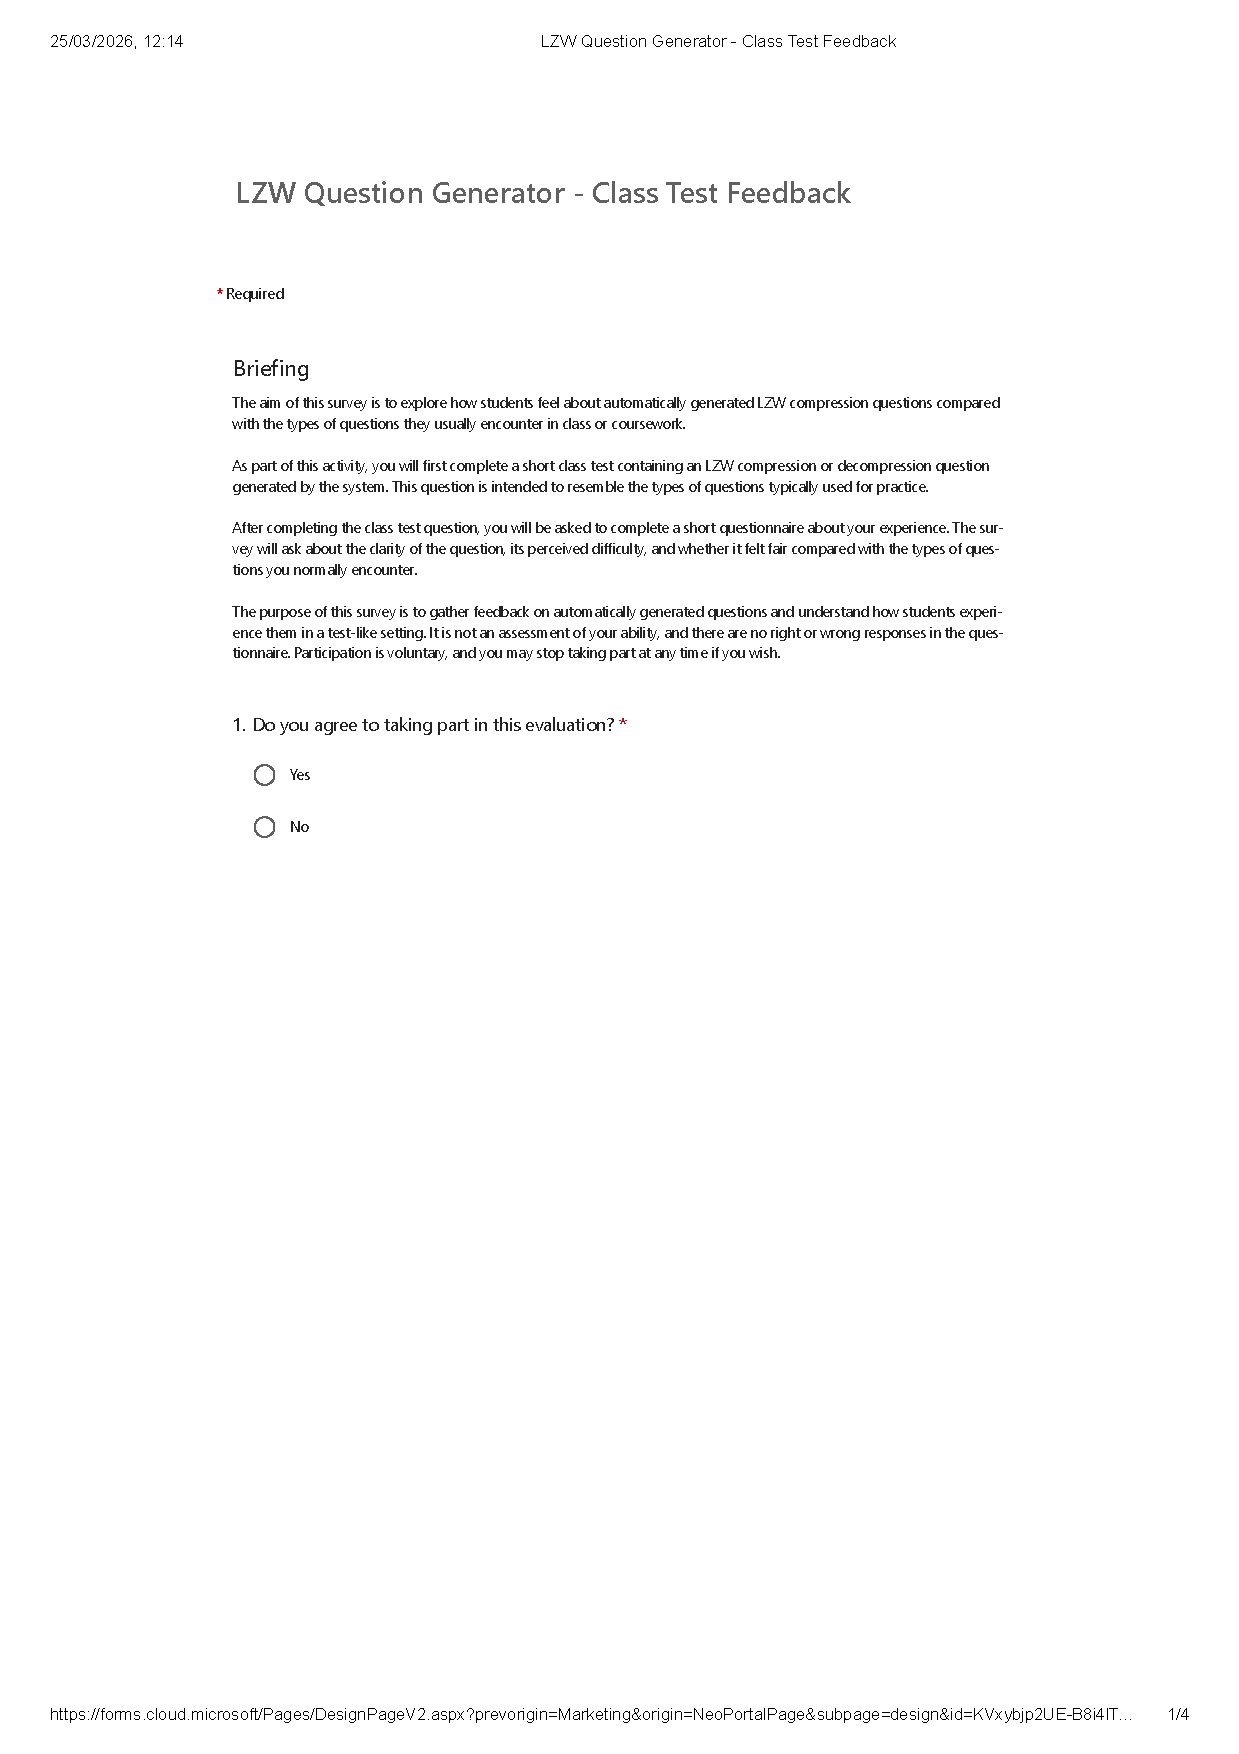
\includepdf[pages=-, scale=0.9, pagecommand={}]{appendices/classtest.pdf}

\chapter{Usability Study Questionnaire}

The following questionnaire was completed by participants in the usability study described in Section~6.3.

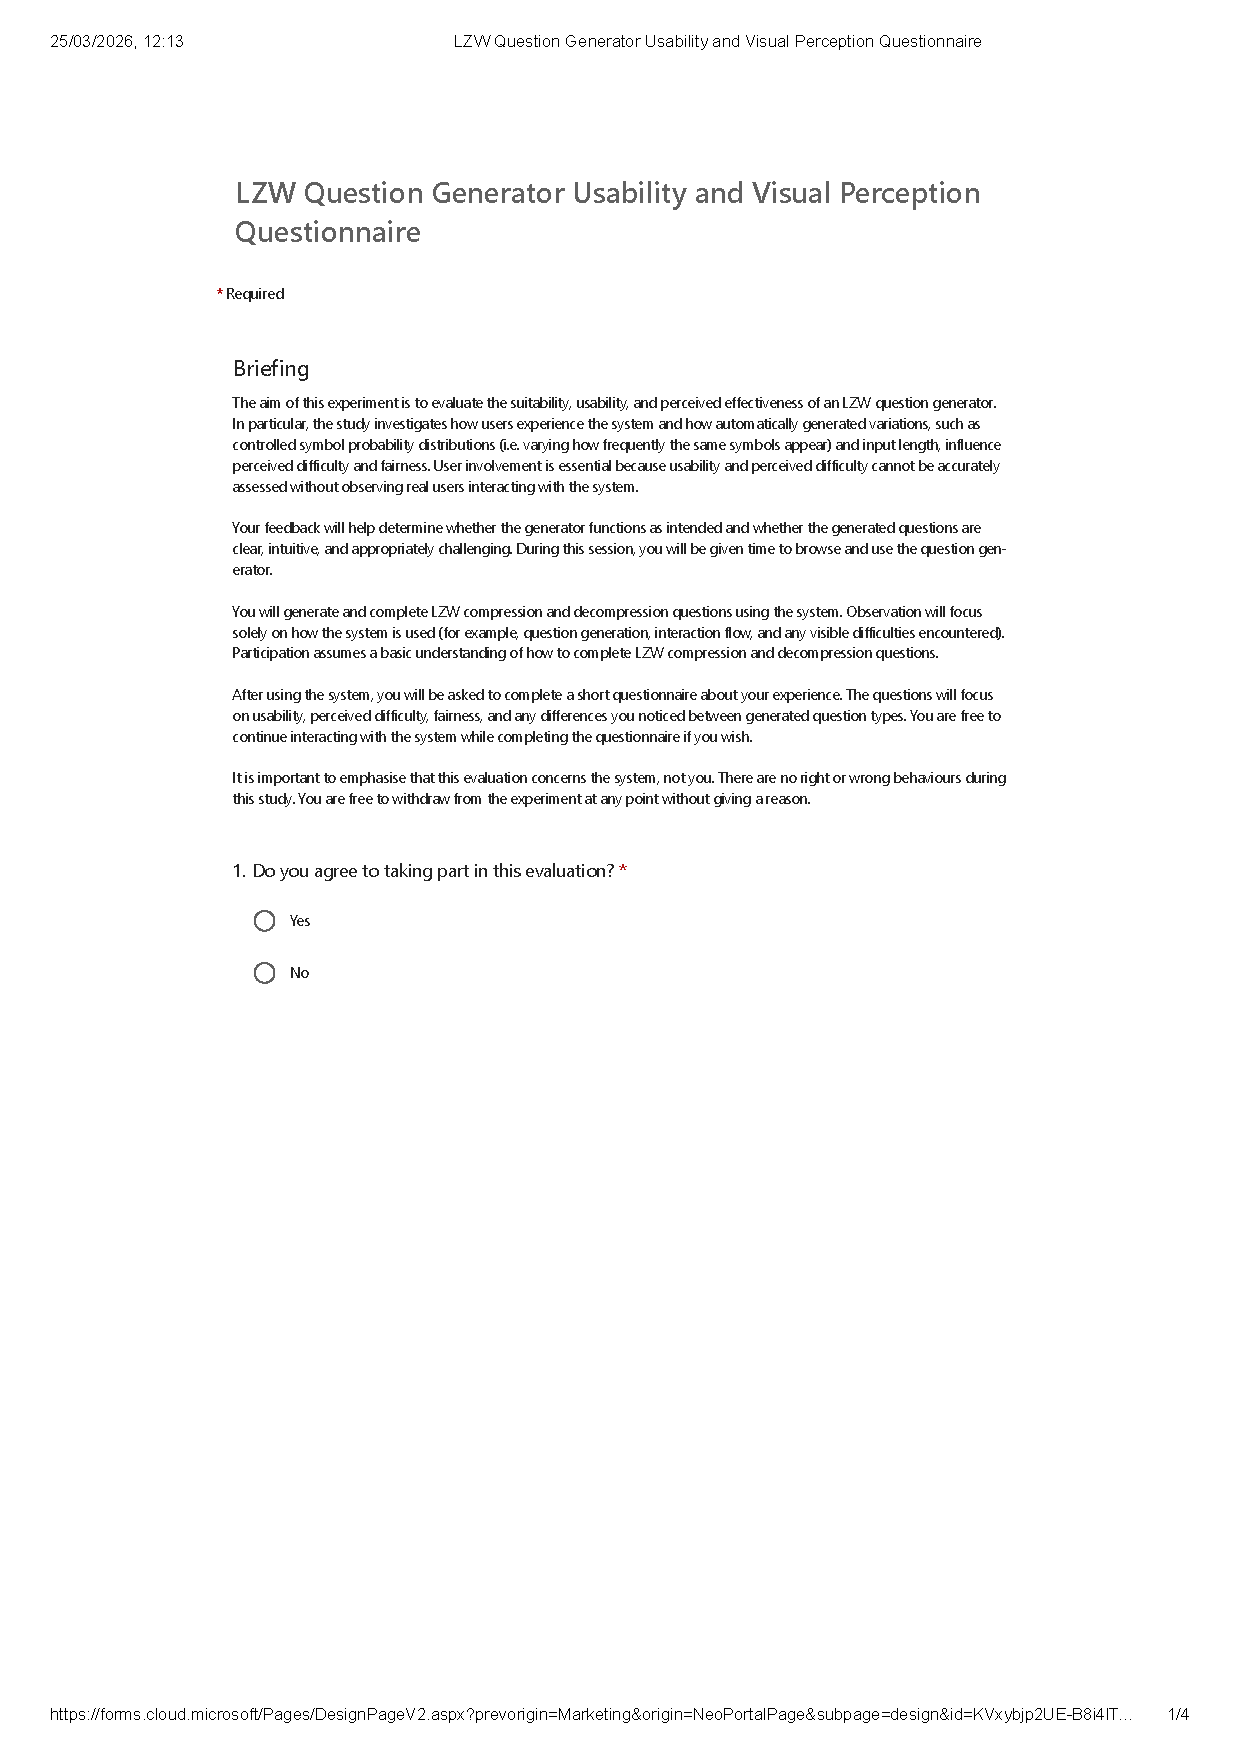
\includepdf[pages=-, scale=0.9, pagecommand={}]{appendices/usability.pdf}


\chapter{User Manual and Source Code Structure}

\section*{Repository Structure}
\begin{verbatim}
Algorithms-Exercise-Generator/
    Implementation/
        LZW_Compression_Generator.py
        LZW_Decompression_Generator.py
        LZW_Figure_Generator.py
        Answers/
        Questions/
    Dissertation/
    Meetings/
    Presentation/
\end{verbatim}

\section*{Requirements}
Python 3.8 or later. No external libraries required. A LaTeX distribution such as MiKTeX (Windows) or MacTeX (Mac) is needed to compile the generated exercise files.

\section*{Running the Compression Generator}
Navigate to the \texttt{Implementation/} directory and run:
\begin{verbatim}
python LZW_Compression_Generator.py
\end{verbatim}
Enter string length (8--30), select a difficulty profile (1 for high entropy, 2 for low entropy), and enter the number of questions to generate. Question sheets are written to \texttt{Questions/} and answer keys to \texttt{Answers/}.

\section*{Running the Decompression Generator}
\begin{verbatim}
python LZW_Decompression_Generator.py
\end{verbatim}
Same prompts as the compression generator, with an additional prompt for special case mode (\texttt{y/n}). When enabled, every generated exercise contains the LZW decompression edge case.

\section*{Compiling Generated Exercises}
Each generated \texttt{.tex} file can be compiled with any standard LaTeX distribution:
\begin{verbatim}
pdflatex lzw_answer_1.tex
\end{verbatim}


\end{appendices}

%==================================================================================================================================
%   BIBLIOGRAPHY   

% The bibliography style is agsm (Harvard)
% The bibliography always appears last, after the appendices.

\bibliographystyle{agsm}

% Force the bibliography not to be numbered
\renewcommand{\thechapter}{0} 
\bibliography{l4proj}

\end{document}
